%%%%%%%%%%%%%%%%%%%%%%% file template.tex %%%%%%%%%%%%%%%%%%%%%%%%%
%
% This is a general template file for the LaTeX package SVJour3
% for Springer journals.          Springer Heidelberg 2010/09/16
%
% Copy it to a new file with a new name and use it as the basis
% for your article. Delete % signs as needed.
%
% This template includes a few options for different layouts and
% content for various journals. Please consult a previous issue of
% your journal as needed.
%
%%%%%%%%%%%%%%%%%%%%%%%%%%%%%%%%%%%%%%%%%%%%%%%%%%%%%%%%%%%%%%%%%%%
%
% First comes an example EPS file -- just ignore it and
% proceed on the \documentclass line
% your LaTeX will extract the file if required
\begin{filecontents*}{example.eps}
%!PS-Adobe-3.0 EPSF-3.0
%%BoundingBox: 19 19 221 221
%%CreationDate: Mon Sep 29 1997
%%Creator: programmed by hand (JK)
%%EndComments
gsave
newpath
  20 20 moveto
  20 220 lineto
  220 220 lineto
  220 20 lineto
closepath
2 setlinewidth
gsave
  .4 setgray fill
grestore
stroke
grestore
\end{filecontents*}
%
\RequirePackage{fix-cm}
%
%\documentclass{svjour3}                     % onecolumn (standard format)
%\documentclass[smallcondensed]{svjour3}     % onecolumn (ditto)
%\documentclass[smallextended]{svjour3}       % onecolumn (second format)
\documentclass[twocolumn]{svjour3}          % twocolumn
%
\smartqed  % flush right qed marks, e.g. at end of proof
%

\usepackage{graphicx}
\usepackage[space]{grffile}
\usepackage{latexsym}
\usepackage{textcomp}
\usepackage{longtable}
\usepackage{tabulary}
\usepackage{booktabs,array,multirow}
\usepackage{amsfonts,amsmath,amssymb}
\providecommand\citet{\cite}
\providecommand\citep{\cite}
\providecommand\citealt{\cite}
\usepackage{url}
\usepackage{hyperref}
\hypersetup{colorlinks=false,pdfborder={0 0 0}}
\usepackage{etoolbox}
\makeatletter
\patchcmd\@combinedblfloats{\box\@outputbox}{\unvbox\@outputbox}{}{%
  \errmessage{\noexpand\@combinedblfloats could not be patched}%
}%
\makeatother
% You can conditionalize code for latexml or normal latex using this.
\newif\iflatexml\latexmlfalse
\providecommand{\tightlist}{\setlength{\itemsep}{0pt}\setlength{\parskip}{0pt}}%

\AtBeginDocument{\DeclareGraphicsExtensions{.pdf,.PDF,.eps,.EPS,.png,.PNG,.tif,.TIF,.jpg,.JPG,.jpeg,.JPEG}}

\usepackage[utf8]{inputenc}
\usepackage[greek,ngerman,english]{babel}


%
% \usepackage{mathptmx}      % use Times fonts if available on your TeX system
%
% insert here the call for the packages your document requires
%\usepackage{latexsym}
% etc.
%
% please place your own definitions here and don't use \def but
% \newcommand{}{}
%
% Insert the name of "your journal" with
% \journalname{myjournal}
%
\newcommand{\truncateit}[1]{\truncate{0.8\textwidth}{#1}}
\newcommand{\scititle}[1]{\title[\truncateit{#1}]{#1}}


\begin{document}

\title{edx Phot1x report template (2016/11)
%\thanks{Grants or other notes
%about the article that should go on the front page should be
%placed here. General acknowledgments should be placed at the end of the article.}
}
%\subtitle{Do you have a subtitle?\\ If so, write it here}

%\titlerunning{Short form of title}        % if too long for running head


\author{Lukas Chrostowski}

\institute{Lukas Chrostowski \at University of British Columbia}

%\authorrunning{Short form of author list} % if too long for running head

%\date{Received: date / Accepted: date}
% The correct dates will be entered by the editor

\maketitle

\selectlanguage{english}
\begin{abstract}
The abstract goes here.
%
\end{abstract}%




\section{Introduction}\label{auto-label-section-729047}

(HTML version)\\

brief motivation for silicon photonics. ~Include references, e.g.,
{[}\hyperref[csl:1]{[1]}{]}. ~\\
objective of your course project.\\

\section{Introduction}
% no \IEEEPARstart
% This demo file is intended to serve as a ``starter file''
% for IEEE conference papers produced under \LaTeX\ using
% IEEEtran.cls version 1.8 and later.
% You must have at least 2 lines in the paragraph with the drop letter
% (should never be an issue)
% I wish you the best of success.

(LaTeX version)

brief motivation for silicon photonics.  Include references, e.g., \hyperref[csl:1]{[1]}.  
objective of your course project.


\section{Theory}\label{auto-label-section-246679}

Short description of the theory relevant to your project. e.g.,
Waveguide compact model, MZI transfer function. ~\\

\section{Modelling and Simulation}\label{auto-label-section-848662}

this should have the compact equation for the waveguide, the transfer
function of our device(s), simulation results, plots of neff/ng vs.
lambda, table with parameter variation (i.e., how FSR is affected by
[?]L), spectrum, waveguide and circuit geometry.\\

Manufacturing variability study (corner analysis, Monte Carlo).\\

\section{Fabrication}\label{fabrication}

Two chips were fabricated in this course. Either report on one dataset,
or on both. Choose the text as appropriate.\\

\subsection{Washington Nanofabrication Facility (WNF) silicon photonics
process:}\label{auto-label-subsection-771002}

The devices were fabricated using 100 keV Electron Beam Lithography
{[}\selectlanguage{english}\hyperref[csl:2]{[2]}{]}. The fabrication used silicon-on-insulator
wafer with 220 nm thick silicon on 3 \selectlanguage{greek}μ\selectlanguage{english}m thick silicon dioxide. The
substrates were 25 mm squares diced from 150 mm wafers. After a solvent
rinse and hot-plate dehydration bake, hydrogen silsesquioxane resist
(HSQ, Dow-Corning XP-1541-006) was spin-coated at 4000 rpm, then
hotplate baked at 80 \selectlanguage{ngerman}°C for 4 minutes. Electron beam lithography was
performed using a JEOL JBX-6300FS system operated at 100 keV energy, 8
nA beam current, and 500 \selectlanguage{greek}µ\selectlanguage{english}m exposure field size. The machine grid used
for shape placement was 1 nm, while the beam stepping grid, the spacing
between dwell points during the shape writing, was 6 nm. An exposure
dose of 2800 \selectlanguage{greek}µ\selectlanguage{english}C/cm2 was used. The resist was developed by immersion in
25\% tetramethylammonium hydroxide for 4 minutes, followed by a flowing
deionized water rinse for 60 s, an isopropanol rinse for 10 s, and then
blown dry with nitrogen. The silicon was removed from unexposed areas
using inductively coupled plasma etching in an Oxford Plasmalab System
100, with a chlorine gas flow of 20 sccm, pressure of 12 mT, ICP power
of 800 W, bias power of 40 W, and a platen temperature of 20 \selectlanguage{ngerman}°C,
resulting in a bias voltage of 185 V. During etching, chips were mounted
on a 100 mm silicon carrier wafer using perfluoropolyether vacuum oil.\\

\subsection{Applied Nanotools, Inc. NanoSOI
process:}\label{auto-label-subsection-267018}

The photonic devices were fabricated using the NanoSOI MPW fabrication
process by Applied Nanotools Inc.
(\url{http://www.appliednt.com/nanosoi}; Edmonton, Canada) which is
based on direct-write 100 keV electron beam lithography technology.
Silicon-on-insulator wafers of 200 mm diameter, 220 nm device thickness
and 2 \selectlanguage{greek}µ\selectlanguage{english}m buffer oxide thickness are used as the base material for the
fabrication. The wafer was pre-diced into square substrates with
dimensions of 25x25 mm, and lines were scribed into the substrate
backsides to facilitate easy separation into smaller chips once
fabrication was complete. After an initial wafer clean using piranha
solution (3:1 H2SO4:H2O2) for 15 minutes and water/IPA rinse, hydrogen
silsesquioxane (HSQ) resist was spin-coated onto the substrate and
heated to evaporate the solvent. The photonic devices were patterned
using a Raith EBPG 5000+ electron beam instrument using a raster step
size of 5 nm. The exposure dosage of the design was corrected for
proximity effects that result from the backscatter of electrons from
exposure of nearby features. Shape writing order was optimized for
efficient patterning and minimal beam drift. After the e-beam exposure
and subsequent development with a tetramethylammonium sulfate (TMAH)
solution, the devices were inspected optically for residues and/or
defects. The chips were then mounted on a 4'' handle wafer and underwent
an anisotropic ICP-RIE etch process using chlorine after qualification
of the etch rate. The resist was removed from the surface of the devices
using a 10:1 buffer oxide wet etch, and the devices were inspected using
a scanning electron microscope (SEM) to verify patterning and etch
quality. A 2.2 \selectlanguage{greek}µ\selectlanguage{english}m oxide cladding was deposited using a plasma-enhanced
chemical vapour deposition (PECVD) process based on tetraethyl
orthosilicate (TEOS) at 300\selectlanguage{ngerman}ºC. Reflectrometry measurements were
performed throughout the process to verify the device layer, buffer
oxide and cladding thicknesses before delivery.\\

\section{Experimental Data}\label{auto-label-section-658796}

To characterize the devices, a custom-built automated test setup
{[}\hyperref[csl:3]{[3]}{]} with automated control software written in
Python was used (\url{http://siepic.ubc.ca/probestation}). ~An Agilent
81600B tunable laser was used as the input source and Agilent 81635A
optical power sensors as the output detectors. The wavelength was swept
from 1500 to 1600 nm in 10 pm steps. ~A polarization maintaining (PM)
fibre was used to maintain the polarization state of the light, to
couple the TE polarization into the grating couplers
{[}\hyperref[csl:4]{[4]}{]}. ~A 90\selectlanguage{ngerman}º rotation was used to inject light into
the TM grating couplers {[}4{]}. ~A polarization maintaining fibre array
was used to couple light in/out of the chip
{[}\href{http://www.plcconnections.com}{www.plcconnections.com}{]}.\\

Plots of experimental data. The following figure was generated using a
built-in Python interpreter!\\\selectlanguage{english}
\begin{figure}[h!]
\begin{center}
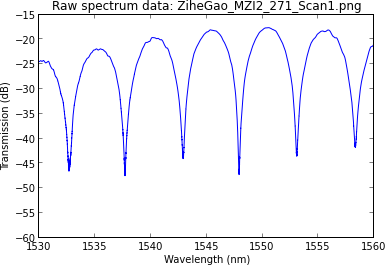
\includegraphics[width=0.70\columnwidth]{figures/download/download}
\caption{{Measured transmission spectrum on a Mach-Zehnder Interferometer with a path length difference of x microns.%
}}
\end{center}
\end{figure}

\section{Analysis}\label{analysis}

Data analysis to extract waveguide group index, etc.\\

Comparison of experimental results with simulations.\\

\section{Conclusion}
The conclusion goes here.



\section{Acknowledgements}\label{auto-label-section-544540}

**(edit according to your use).**\\

I/We acknowledge the edX UBCx Phot1x Silicon Photonics Design,
Fabrication and Data Analysis course, which is supported by the Natural
Sciences and Engineering Research Council of Canada (NSERC) Silicon
Electronic-Photonic Integrated Circuits (SiEPIC) Program.
The~devices~were fabricated by Richard Bojko at the University of
Washington Washington Nanofabrication Facility, part of the National
Science Foundation's National Nanotechnology Infrastructure Network
(NNIN), and Cameron Horvath at Applied Nanotools, Inc. Enxiao
Luan~performed the measurements at The University of British Columbia.
We acknowledge Lumerical Solutions, Inc., Mathworks, Mentor Graphics,
Python, and KLayout for the design software. ~

\selectlanguage{english}
\FloatBarrier
\section*{References}\sloppy
\phantomsection
\label{csl:1}1. Chrostowski L, Hochberg M (2015) {Silicon Photonics Design}. Cambridge University Press ({CUP})

\phantomsection
\label{csl:2}2. Bojko RJ, Li J, He L, et al. (2011) {Electron beam lithography writing strategies for low loss high confinement silicon optical waveguides}. Journal of Vacuum Science {\&} Technology B: Microelectronics and Nanometer Structures 29:06F309. \url{https://doi.org/10.1116/1.3653266}

\phantomsection
\label{csl:3}3. Chrostowski L, Hochberg M {Testing and packaging}. In: Silicon Photonics Design. Cambridge University Press ({CUP}), pp 381–405

\phantomsection
\label{csl:4}4. Wang Y, Wang X, Flueckiger J, et al. (2014) {Focusing sub-wavelength grating couplers with low back reflections for rapid prototyping of silicon photonic circuits}. Opt Express 22:20652. \url{https://doi.org/10.1364/oe.22.020652}

\end{document}

